% tikz/trees.tex -- figure: the built-in tree topologies (input from sections/02_setup.tex).
% Node layout follows ttn/tree.py: binary_tree, mps_tree (root = last core), ht_tree.
% Sites are numbered 1..N here (0..N-1 in the code).
\tikzset{
  ttn/core/.style={circle, draw=MidnightBlue!75!black, fill=MidnightBlue!12, line width=0.6pt,
                   minimum size=3.6mm, inner sep=0pt},
  ttn/root/.style={ttn/core, fill=MidnightBlue!60},
  ttn/bond/.style={line width=1.2pt, black!80},
  ttn/phys/.style={line width=0.6pt, black!55},
  ttn/site/.style={font=\scriptsize, inner sep=1pt, text=black!75},
}
\begin{figure}[t]
  \centering
  \begin{subfigure}[b]{0.37\textwidth}
    \centering
    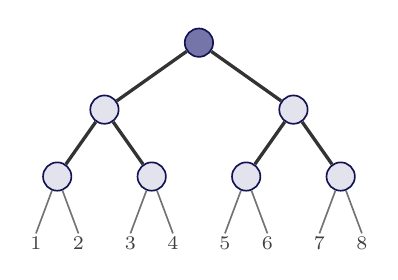
\begin{tikzpicture}[x=6mm, y=8.5mm]
      \foreach \j in {1,...,4} \node[ttn/core] (b\j) at ({2*\j-1}, 0) {};
      \node[ttn/core] (m1) at (2, 1) {};
      \node[ttn/core] (m2) at (6, 1) {};
      \node[ttn/root] (r) at (4, 2) {};
      \draw[ttn/bond] (b1) -- (m1) -- (b2)  (b3) -- (m2) -- (b4)  (m1) -- (r) -- (m2);
      \foreach \j in {1,...,4} {
        \pgfmathtruncatemacro{\sa}{2*\j-1}
        \pgfmathtruncatemacro{\sb}{2*\j}
        \draw[ttn/phys] (b\j) -- ++(-0.45,-0.85) node[ttn/site, below] {\sa};
        \draw[ttn/phys] (b\j) -- ++(0.45,-0.85) node[ttn/site, below] {\sb};
      }
    \end{tikzpicture}
    \caption{binary, $\Ns=8$, $\Kc=7$}
    \label{fig:trees-binary}
  \end{subfigure}%
  \hfill
  \begin{subfigure}[b]{0.37\textwidth}
    \centering
    \begin{tikzpicture}[x=6mm, y=8.5mm]
      \foreach \k in {1,...,7} \node[ttn/core] (c\k) at (\k, 0) {};
      \node[ttn/root] (c8) at (8, 0) {};
      \foreach \k [evaluate=\k as \kn using int(\k+1)] in {1,...,7}
        \draw[ttn/bond] (c\k) -- (c\kn);
      \foreach \k in {1,...,8}
        \draw[ttn/phys] (c\k) -- ++(0,-0.85) node[ttn/site, below] {\k};
      \node[font=\scriptsize, above=1.5pt] at ($(c4)!0.5!(c5)$) {$\bd{4}$};
    \end{tikzpicture}
    \caption{MPS, $\Ns=8$, $\Kc=8$}
    \label{fig:trees-mps}
  \end{subfigure}%
  \hfill
  \begin{subfigure}[b]{0.22\textwidth}
    \centering
    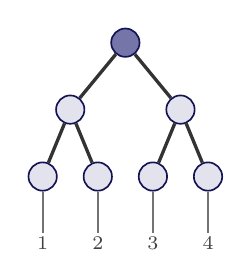
\begin{tikzpicture}[x=7mm, y=8.5mm]
      \foreach \i in {1,...,4} \node[ttn/core] (l\i) at (\i, 0) {};
      \node[ttn/core] (h1) at (1.5, 1) {};
      \node[ttn/core] (h2) at (3.5, 1) {};
      \node[ttn/root] (r) at (2.5, 2) {};
      \draw[ttn/bond] (l1) -- (h1) -- (l2)  (l3) -- (h2) -- (l4)  (h1) -- (r) -- (h2);
      \foreach \i in {1,...,4}
        \draw[ttn/phys] (l\i) -- ++(0,-0.85) node[ttn/site, below] {\i};
    \end{tikzpicture}
    \caption{HT, $\Ns=4$, $\Kc=7$}
    \label{fig:trees-ht}
  \end{subfigure}
  \caption{The built-in tree topologies (\cref{tab:trees}). Circles are cores $\G{v}$; the shaded
    core is the root, whose parent leg (dimension one, the scalar output) is not drawn. Thick lines
    are bonds: the edge $\edge{v}$ between core $v$ and its parent has dimension $\bd{v}$ (one label
    shown in (b), where cores are numbered $1,\dots,8$ from the left). Thin dangling lines are
    physical legs, labelled by their site $i$ (dimension $\pd[i]$).}
  \label{fig:trees}
\end{figure}
